%% LyX 2.4.4 created this file.  For more info, see https://www.lyx.org/.
%% Do not edit unless you really know what you are doing.
\documentclass[english]{article}
\usepackage[T1]{fontenc}
\usepackage[latin9]{inputenc}
\usepackage{units}
\usepackage{enumitem}
\usepackage{amsmath}
\usepackage{amsthm}
\usepackage{cancel}
\usepackage{geometry}
\geometry{verbose,tmargin=1in,bmargin=1in,lmargin=1in,rmargin=1in}
\PassOptionsToPackage{normalem}{ulem}
\usepackage{ulem}

\makeatletter

%%%%%%%%%%%%%%%%%%%%%%%%%%%%%% LyX specific LaTeX commands.
%% Because html converters don't know tabularnewline
\providecommand{\tabularnewline}{\\}

%%%%%%%%%%%%%%%%%%%%%%%%%%%%%% Textclass specific LaTeX commands.
\numberwithin{equation}{section}
\numberwithin{figure}{section}
\newlength{\lyxlabelwidth}      % auxiliary length 

%%%%%%%%%%%%%%%%%%%%%%%%%%%%%% User specified LaTeX commands.
\usepackage{hyperref}
\usepackage[usenames,dvipsnames,table]{xcolor} %adds additional color options
\hypersetup{colorlinks=true, urlcolor=black,linkcolor=black}

\usepackage{fancyhdr}
\usepackage{lastpage}
\pagestyle{fancy}
\usepackage{enumitem}
\usepackage{ifthen}
%sets math fonts to be more readable
\everymath=\expandafter{\the\everymath\displaystyle}
%\DeclareMathSizes{10}{10}{10}{10}
\usepackage{multicol}

\usepackage{tikz}
\usetikzlibrary{plotmarks}
\usepackage{pgfplots}
\pgfplotsset{compat=newest}

\usepackage{calc}
\usepackage[nomessages]{fp}

\usepackage{advdate}    % Advancing/saving dates
\usepackage{datetime}   % Dates formatting
\usepackage{datenumber} % Counters for dates

\usepackage{fancybox} %%ovalbox and fancy box settings

\usepackage[outline]{contour}  %allows text halos
\usepackage{colortbl}


\usepackage[super]{nth} %easy 1st, 2nd, etc

\usepackage{forest} %%for tree diagram

%%data for histogram%%
\begin{filecontents}{hist1_data.csv} 
dist 
3
1
0
4
1
3
2
2
0
2
0
2
2
1
4
3
1
1
3
4
2
1
3
0
1
0
2
5
1
2
3
0
0
1
2
3
1
2
0
2
\end{filecontents}

%%data for histogra: cal per cereal%%
\begin{filecontents}{hist_data_cereal.csv} 
dist 
3.7
3.6
3.6
4.0
4.0
3.6
3.8
3.7
4.1
3.9
3.9
3.3
3.5
3.6
3.9
4.0
\end{filecontents}
% Added by lyx2lyx
\setlength{\parskip}{\smallskipamount}
\setlength{\parindent}{0pt}

\makeatother

\usepackage{babel}
\begin{document}
\renewcommand{\author}{Dr.\,James Ashe}

\newcommand{\classNum}{107}

\newcommand{\classSec}{7}

\newcommand{\nameType}{Solutions}

\newcommand{\examType}{Final Exam Review}

\renewcommand{\date}{}

%%First page's header%%%%%%%%%%%%%%%%%%%%%%
\fancypagestyle{firststyle} %%header settings for first pagr
{
	\fancyhead[L]{MTH \classNum{}(\classSec{}) \author{}\\
	\textbf{\examType{}} \date{}}
	\fancyhead[C]{\textbf{\nameType}}
	\setlength{\headsep}{14pt}
}
%%%%%%%%%%%%%%%%%%%%%%%%%%%%%%%%%%%%%%%%%%

%%Next page's header%%%%%%%%%%%%%%%%%%%%%%%
%\setlist{nolistsep}
\lhead{MTH \classNum{}(\classSec{})} 
\chead{\textbf{\nameType}} 
\cfoot{\thepage{}~of~\pageref{LastPage}} 
\setlength{\headsep}{5pt} 
%%%%%%%%%%%%%%%%%%%%%%%%%%%%%%%%%%%%%%%%%%%

%%Various settings; see the preamble for other settings%%%%%
%%\setenumerate[0]{leftmargin=12pt,itemindent=0pt,labelwidth=0pt}
%\setlist[2]{noitemsep}
%\setlist{nosep}
%\setlist{itemsep=-3pt,topsep=-2pt}
\renewcommand{\labelenumi}{\textbf{\arabic{enumi}.}}
\renewcommand{\labelenumii}{\textbf{\alph{enumii}.}}
\thispagestyle{firststyle}
%%%%%%%%%%%%%%%%%%%%%%%%%%%%%%%%%%%%%%%%%%
\newcommand{\xmax}{10}
\newcommand{\xmin}{-10}
\newcommand{\xstep}{0} %must be xmin+n
\newcommand{\ymax}{10}
\newcommand{\ymin}{-10}
\newcommand{\ystep}{0} %must be ymin+n

\newcommand{\xspace}{\hspace*{40pt}}
\newcommand{\yspace}{\vspace*{0cm}}
\newcommand{\rowColor}{gray!35}
\large\newcommand{\T}{\textcolor{green}{\contour{black}{T}}}
\newcommand{\F}{\textcolor{red}{\contour{black}{F}}}

\newcommand{\gauss}[2]{1/(#2*sqrt(2*pi))*exp(-((x-#1)^2)/(2*#2^2))}

\newcommand{\normalcdf}[4]{ %mean,std,z-left,z-right
\begin{tikzpicture}[scale=1.0]

\pgfmathsetmacro{\mn}{#1}
\pgfmathsetmacro{\sd}{#2}
\pgfmathsetmacro{\za}{#1+#2*1}
\pgfmathsetmacro{\zb}{#1+#2*2}
\pgfmathsetmacro{\zc}{#1+#2*3}

\pgfmathsetmacro{\zna}{#1-#2*1}
\pgfmathsetmacro{\znb}{#1-#2*2}
\pgfmathsetmacro{\znc}{#1-#2*3}

\pgfmathsetmacro{\zleft}{#3}
\pgfmathsetmacro{\zright}{#4}
\pgfmathsetmacro{\zsL}{(#3-#1)/#2} %z-score
\pgfmathsetmacro{\zsR}{(#4-#1)/#2} %z-score
\pgfmathsetmacro{\xCenter}{\zsL/2.5+\zsR/2.5} %center using z-score
\pgfmathsetmacro{\yCenter}{((1/(1*sqrt(2*pi))*exp(-((\xCenter-0)^2)/(2*1^2)))/2}
\pgfkeys{/pgf/fpu} %for large numbers
\pgfmathparse{100*(1/(1 + exp(-0.07056*((\zsR-0)/1)^3 - 1.5976*(\zsR-0)/1))-1/(1 + exp(-0.07056*((\zsL-0)/1)^3 - 1.5976*(\zsL-0)/1)))} %area from z-left to z-right
\edef\area{\pgfmathresult} 
\pgfkeys{/pgf/fpu=false}

\scriptsize
\begin{axis}[ 
	no markers, 
	domain=0:10, 
	%samples=100, 
	axis lines*=left, 
	%xlabel=Standard deviations, 
	%ylabel=Frequency, 
	height=2.5cm, %change/remove this scaling to get 1:1 pic
	width=5.5cm, 
	hide y axis,
	%ticks=none,
	xtick={-3,-2,-1,0,1,2,3},
	xticklabels={\pgfmathprintnumber[precision=0]{\znc},\pgfmathprintnumber[precision=2]{\znb},\pgfmathprintnumber[precision=2]{\zna},#1,\pgfmathprintnumber[precision=0]{\za},\pgfmathprintnumber[precision=2]{\zb},\pgfmathprintnumber[precision=2]{\zc}},
	%xticklabels={-25, -15, -5, 5, 15, 25, 35},
	%ytick=empty, 
	enlargelimits=false, 
	clip=false, 
	axis on top, 
	%grid = major
	]

	\addplot [fill=blue!35, draw=red,  domain=\zsL:\zsR] {\gauss{0}{1}} \closedcycle;
		\node (arrowEnd) at (axis cs: \xCenter, \yCenter) {};
	\addplot [draw, thick, smooth, domain=-3:3] {\gauss{0}{1}} \closedcycle;
		\node[anchor=south east] (arrowStart) at (current bounding box.east) {\pgfmathprintnumber[fixed,precision=1]{\area}\%};
	\draw[->,thick,black] (arrowStart) to (arrowEnd);
	
	%\addplot [fill=orange!20, draw=none, domain=2:3] {\gauss{0}{1}} \closedcycle; 
	%\addplot [fill=blue!20, draw=none, domain=-2:-1] {\gauss{0}{1}} \closedcycle; 
	%\addplot [fill=blue!20, draw=none, domain=1:2] {\gauss{0}{1}} \closedcycle; 
	%\only<1->{\node[above] at (axis cs: -0.5, 0.025) {$34.1\%$};} 
	%\only<1->{\node[above] at (axis cs: 0.5, 0.025) {$34.1\%$};} 
	%\only<1->{\node[above] at (axis cs: -1.5, 0.025) {$13.6\%$};}
	%\only<1->{\node[above] at (axis cs: 1.5, 0.025) {$13.6\%$};}
	%\only<1->{\node[above] at (axis cs: 2.5, 0.05) {$2.1\%$};}
	%\only<1->{\node[above] at (axis cs: -2.5, 0.05) {$2.1\%$};}
	%\only<1->{ \addplot[<->,black,very thick] coordinates {(-1,0.4) (1,0.4)};} 
	%\only<1->{\node[above] at (axis cs: 0, 0.4) {$68.2\%$};} 
	%\only<1->{\addplot[<->,black,very thick] coordinates {(-2,0.3) (2,0.3)};}
	%\only<1->{\node[above] at (axis cs: 0, 0.3) {$95.4\%$};}
	%\only<1->{\addplot[<->,black, very thick] coordinates {(-3,0.2) (3,0.2)};} 
	%\only<1->{\node[above] at (axis cs: 0, 0.2) {$99.7\%$};}
	\end{axis} 
\end{tikzpicture}
}

\newcommand{\normalpdf}[5]{ %mean,std,z-left,z-right
\begin{tikzpicture}[scale=1]

\pgfmathsetmacro{\mn}{#1}
\pgfmathsetmacro{\sd}{#2}
\pgfmathsetmacro{\za}{#1+#2*1}
\pgfmathsetmacro{\zb}{#1+#2*2}
\pgfmathsetmacro{\zc}{#1+#2*3}

\pgfmathsetmacro{\zna}{#1-#2*1}
\pgfmathsetmacro{\znb}{#1-#2*2}
\pgfmathsetmacro{\znc}{#1-#2*3}

\pgfmathsetmacro{\zleft}{#3}
\pgfmathsetmacro{\zright}{#4}
\pgfmathsetmacro{\zsL}{(#3-#1)/#2} %z-score
\pgfmathsetmacro{\zsR}{(#4-#1)/#2} %z-score
\pgfmathsetmacro{\zsV}{(#5-#1)/#2} %z-score
\pgfmathsetmacro{\xCenter}{\zsL/2.5+\zsR/2.5} %center using z-score
\pgfmathsetmacro{\yCenter}{((1/(1*sqrt(2*pi))*exp(-((\xCenter-0)^2)/(2*1^2)))/2}
\pgfkeys{/pgf/fpu} %for large numbers
\pgfmathparse{100*(1/(1 + exp(-0.07056*((\zsR-0)/1)^3 - 1.5976*(\zsR-0)/1))-1/(1 + exp(-0.07056*((\zsL-0)/1)^3 - 1.5976*(\zsL-0)/1)))} %area from z-left to z-right
\edef\area{\pgfmathresult} 
\pgfkeys{/pgf/fpu=false}

\scriptsize
\begin{axis}[ 
	no markers, 
	domain=0:10, 
	%samples=100, 
	axis lines*=left, 
	%xlabel=Standard deviations, 
	%ylabel=Frequency, 
	height=2.5cm, %change/remove this scaling to get 1:1 pic
	width=5.5cm, 
	hide y axis,
	%ticks=none,
	xtick={\zsV},
	xticklabels={\pgfmathprintnumber[precision=2]{#5}},
	%xticklabels={-25, -15, -5, 5, 15, 25, 35},
	%ytick=empty, 
	enlargelimits=false, 
	clip=false, 
	axis on top, 
	%grid = major
	]

	\addplot [fill=blue!35, draw=red,  domain=\zsL:\zsR] {\gauss{0}{1}} \closedcycle;
		\node (arrowEnd) at (axis cs: \xCenter, \yCenter) {};
	\addplot [draw, thick, smooth, domain=-3:3] {\gauss{0}{1}} \closedcycle;
		\node[anchor=south east] (arrowStart) at (current bounding box.east) {\pgfmathprintnumber[fixed,precision=1]{\area}\%};
	\draw[->,thick,black] (arrowStart) to (arrowEnd);
	
	%\addplot [fill=orange!20, draw=none, domain=2:3] {\gauss{0}{1}} \closedcycle; 
	%\addplot [fill=blue!20, draw=none, domain=-2:-1] {\gauss{0}{1}} \closedcycle; 
	%\addplot [fill=blue!20, draw=none, domain=1:2] {\gauss{0}{1}} \closedcycle; 
	%\only<1->{\node[above] at (axis cs: -0.5, 0.025) {$34.1\%$};} 
	%\only<1->{\node[above] at (axis cs: 0.5, 0.025) {$34.1\%$};} 
	%\only<1->{\node[above] at (axis cs: -1.5, 0.025) {$13.6\%$};}
	%\only<1->{\node[above] at (axis cs: 1.5, 0.025) {$13.6\%$};}
	%\only<1->{\node[above] at (axis cs: 2.5, 0.05) {$2.1\%$};}
	%\only<1->{\node[above] at (axis cs: -2.5, 0.05) {$2.1\%$};}
	%\only<1->{ \addplot[<->,black,very thick] coordinates {(-1,0.4) (1,0.4)};} 
	%\only<1->{\node[above] at (axis cs: 0, 0.4) {$68.2\%$};} 
	%\only<1->{\addplot[<->,black,very thick] coordinates {(-2,0.3) (2,0.3)};}
	%\only<1->{\node[above] at (axis cs: 0, 0.3) {$95.4\%$};}
	%\only<1->{\addplot[<->,black, very thick] coordinates {(-3,0.2) (3,0.2)};} 
	%\only<1->{\node[above] at (axis cs: 0, 0.2) {$99.7\%$};}
	\end{axis} 
\end{tikzpicture}
}\newcommand{\normalpdfB}[4]{ %mean,std,z-left,z-right
\begin{tikzpicture}[scale=1]

\pgfmathsetmacro{\mn}{#1}
\pgfmathsetmacro{\sd}{#2}
\pgfmathsetmacro{\za}{#1+#2*1}
\pgfmathsetmacro{\zb}{#1+#2*2}
\pgfmathsetmacro{\zc}{#1+#2*3}

\pgfmathsetmacro{\zna}{#1-#2*1}
\pgfmathsetmacro{\znb}{#1-#2*2}
\pgfmathsetmacro{\znc}{#1-#2*3}

\pgfmathsetmacro{\zleft}{#3}
\pgfmathsetmacro{\zright}{#4}
\pgfmathsetmacro{\zsL}{(#3-#1)/#2} %z-score
\pgfmathsetmacro{\zsR}{(#4-#1)/#2} %z-score
\pgfmathsetmacro{\xCenter}{\zsL/2.5+\zsR/2.5} %center using z-score
\pgfmathsetmacro{\yCenter}{((1/(1*sqrt(2*pi))*exp(-((\xCenter-0)^2)/(2*1^2)))/2}
\pgfkeys{/pgf/fpu} %for large numbers
\pgfmathparse{100*(1/(1 + exp(-0.07056*((\zsR-0)/1)^3 - 1.5976*(\zsR-0)/1))-1/(1 + exp(-0.07056*((\zsL-0)/1)^3 - 1.5976*(\zsL-0)/1)))} %area from z-left to z-right
\edef\area{\pgfmathresult} 
\pgfkeys{/pgf/fpu=false}

\scriptsize
\begin{axis}[ 
	no markers, 
	domain=0:10, 
	%samples=100, 
	axis lines*=left, 
	%xlabel=Standard deviations, 
	%ylabel=Frequency, 
	height=2.5cm, %change/remove this scaling to get 1:1 pic
	width=5.5cm, 
	hide y axis,
	%ticks=none,
	xtick={\zsL,\zsR},
	xticklabels={\pgfmathprintnumber[precision=2]{\zsL},\pgfmathprintnumber[precision=2]{\zsR}},
	%xticklabels={-25, -15, -5, 5, 15, 25, 35},
	%ytick=empty, 
	enlargelimits=false, 
	clip=false, 
	axis on top, 
	%grid = major
	]

	\addplot [fill=blue!35, draw=red,  domain=\zsL:\zsR] {\gauss{0}{1}} \closedcycle;
		\node (arrowEnd) at (axis cs: \xCenter, \yCenter) {};
	\addplot [draw, thick, smooth, domain=-3:3] {\gauss{0}{1}} \closedcycle;
		\node[anchor=south east] (arrowStart) at (current bounding box.east) {\pgfmathprintnumber[fixed,precision=1]{\area}\%};
	\draw[->,thick,black] (arrowStart) to (arrowEnd);
	
	%\addplot [fill=orange!20, draw=none, domain=2:3] {\gauss{0}{1}} \closedcycle; 
	%\addplot [fill=blue!20, draw=none, domain=-2:-1] {\gauss{0}{1}} \closedcycle; 
	%\addplot [fill=blue!20, draw=none, domain=1:2] {\gauss{0}{1}} \closedcycle; 
	%\only<1->{\node[above] at (axis cs: -0.5, 0.025) {$34.1\%$};} 
	%\only<1->{\node[above] at (axis cs: 0.5, 0.025) {$34.1\%$};} 
	%\only<1->{\node[above] at (axis cs: -1.5, 0.025) {$13.6\%$};}
	%\only<1->{\node[above] at (axis cs: 1.5, 0.025) {$13.6\%$};}
	%\only<1->{\node[above] at (axis cs: 2.5, 0.05) {$2.1\%$};}
	%\only<1->{\node[above] at (axis cs: -2.5, 0.05) {$2.1\%$};}
	%\only<1->{ \addplot[<->,black,very thick] coordinates {(-1,0.4) (1,0.4)};} 
	%\only<1->{\node[above] at (axis cs: 0, 0.4) {$68.2\%$};} 
	%\only<1->{\addplot[<->,black,very thick] coordinates {(-2,0.3) (2,0.3)};}
	%\only<1->{\node[above] at (axis cs: 0, 0.3) {$95.4\%$};}
	%\only<1->{\addplot[<->,black, very thick] coordinates {(-3,0.2) (3,0.2)};} 
	%\only<1->{\node[above] at (axis cs: 0, 0.2) {$99.7\%$};}
	\end{axis} 
\end{tikzpicture}
}\small
\begin{enumerate}[resume]
\item Using the symbolic representations\\
\begin{tabular}{rl}
$b$: & I ride a bicycle to school.\tabularnewline
$s$: & It is snowing.\tabularnewline
$r$: & It is raining. \tabularnewline
\end{tabular}\\
express the following statements in symbolic form.

\begin{enumerate}
\item It is raining and I rode my bicycle to school.

\begin{enumerate}
\item []$r\wedge b$\yspace
\end{enumerate}
\item If it is raining or snowing, then I will not ride my bicycle to school.

\begin{enumerate}
\item []$(r\vee s)\rightarrow\sim b$\yspace
\end{enumerate}
\end{enumerate}
\item Using the statement, ``If your order is over \$50, then you will
not have to pay shipping fees.'' and parts (a), (b), and (c) below,
complete the following:\emph{}\\
\emph{}

\begin{enumerate}
\item If $\mbox{you do not have to pay shipping fees}$ then $\mbox{your order is over \$50}$.
$\sim p\rightarrow o$
\item If $\mbox{your order is not over \$50}$ then $\mbox{you have to pay shipping fees}$.
$\sim o\rightarrow p$
\item If $\mbox{you have to pay shipping fees}$ then $\mbox{your order is not over \$50}$.
$p\rightarrow\sim o$
\item []Now write the statement as: $o\rightarrow\sim p$ 
\item []Identify the converse of the statement. The converse is $\sim p\rightarrow o$
\textbf{(a)}
\item []Identify the inverse of the statement. The inverse is $\sim o\rightarrow\sim(\sim p)$
\textbf{(b)}
\item []Identify the contrapositive of the statement. The contrapositive
is $p\rightarrow\sim o$ \textbf{(c)}\vfill
\end{enumerate}
\item For parts \ref{enu:one}-\ref{enu:last}, identify the negation of
the provided statement.\newcommand{\negate}{students~}\begin{multicols}{2}

\begin{enumerate}
\item \label{enu:one}\renewcommand{\negate}{students~}Some \negate are
taking Math 107.

\begin{enumerate}
\item [(a)]All \negate are taking Math 107.
\item [\ovalbox{(b)}]No \negate are taking Math 107.
\item [(c)]Some \negate are not taking Math 107.
\item [(d)]Some \negate are taking Math 107.
\item []%
\begin{tabular}{ccc}
 & \emph{negate} & \tabularnewline
all & $\longleftrightarrow$ & some\tabularnewline
none & $\leftrightarrow$ & \tabularnewline
 &  & \tabularnewline
\end{tabular}\vfill
\end{enumerate}
\item \renewcommand{\negate}{players~}All \negate need to attend practice.

\begin{enumerate}
\item [(a)]All \negate need to attend practice.
\item [(b)]No \negate need to attend practice.
\item [\ovalbox{(c)}]Some \negate do not need to attend practice.
\item [(d)]Some \negate need to attend practice.\vfill\columnbreak
\end{enumerate}
\item \renewcommand{\negate}{professors~}No \negate know how to read.

\begin{enumerate}
\item [(a)]All \negate know how to read.
\item [(b)]No \negate know how to read.
\item [(c)]Some \negate do not know how to read.
\item [\ovalbox{(d)}]Some \negate know how to read.\vfill
\end{enumerate}
\item \label{enu:last}\renewcommand{\negate}{students~}Some \negate are
going to lunch.

\begin{enumerate}
\item [(a)]All \negate are going to lunch.
\item [\ovalbox{(b)}]No \negate are going to lunch.
\item [(c)]Some \negate are not going to lunch.
\item [(d)]Some \negate are going to lunch.\vfill
\end{enumerate}
\end{enumerate}
\end{multicols}\vfill
\item Use a truth table to determine if the following arguments are valid.

\begin{enumerate}
\item \vspace{-25pt}%
\begin{tabular}{rll}
 &  & \tabularnewline
 &  & \tabularnewline
$b$: & You buy the bike. & 1. You buy the bike or the tent.\tabularnewline
$t$: & You buy the tent. & 2. You buy the bike.\tabularnewline
\cline{3-3}
 &  & Therefore, you do not buy the tent.\tabularnewline
\end{tabular}\\
\begin{tabular}{c|c|c|c|c|c|c}
\multicolumn{1}{c}{} & \multicolumn{1}{c}{} & \multicolumn{1}{c}{\xspace} & \multicolumn{1}{c}{\xspace} & \multicolumn{1}{c}{\xspace} & \multicolumn{1}{c}{\xspace} & \xspace\tabularnewline
\multicolumn{1}{c}{} & \multicolumn{1}{c}{} & \multicolumn{1}{c}{\ovalbox{$1$}} & \multicolumn{1}{c}{\ovalbox{$2$}} & \multicolumn{1}{c}{} & \multicolumn{1}{c}{\ovalbox{$c$}} & \ovalbox{Argument}\tabularnewline
$b$ & $t$ & $b\vee t$ & $b$ & $1 \wedge 2$ & $\sim t$ & $\left(1\wedge2\right)\rightarrow c$\tabularnewline
\hline 
\hline 
\rowcolor{\rowColor}T & T & \T & \T & \T & \F & \fbox{\F}\tabularnewline
\hline 
T & F & \T & \T & \T & \T & \T\tabularnewline
\hline 
\rowcolor{\rowColor}F & T & \T & \F & \F & \F & \T\tabularnewline
\hline 
F & F & \F & \F & \F & \T & \T\tabularnewline
\end{tabular}

\begin{enumerate}
\item []The argument is not always true so it is,\textbf{ invalid}\yspace\newpage
\end{enumerate}
\item \vspace{-25pt} %
\begin{tabular}{rll}
 &  & \tabularnewline
 &  & \tabularnewline
$r$: & You register early. & 1. If you register early, then you will receive a discount.\tabularnewline
$d$: & You receive a discount. & 2. You register early.\tabularnewline
\cline{3-3}
 &  & Therefore, you will receive a discount.\tabularnewline
\end{tabular}\\
\begin{tabular}{c|c|c|c|c|c|c}
\multicolumn{1}{c}{} & \multicolumn{1}{c}{} & \multicolumn{1}{c}{\xspace} & \multicolumn{1}{c}{\xspace} & \multicolumn{1}{c}{\xspace} & \multicolumn{1}{c}{\xspace} & \xspace\tabularnewline
\multicolumn{1}{c}{} & \multicolumn{1}{c}{} & \multicolumn{1}{c}{\ovalbox{$1$}} & \multicolumn{1}{c}{\ovalbox{$2$}} & \multicolumn{1}{c}{} & \multicolumn{1}{c}{\ovalbox{$c$}} & \ovalbox{Argument}\tabularnewline
$r$ & $d$ & $r\rightarrow d$ & $r$ & $1 \wedge 2$ & $r$ & $\left(1\wedge2\right)\rightarrow c$\tabularnewline
\hline 
\hline 
\rowcolor{\rowColor}T & T & \T & \T & \T & \T & \T\tabularnewline
\hline 
T & F & \F & \T & \F & \T & \T\tabularnewline
\hline 
\rowcolor{\rowColor}F & T & \T & \F & \F & \F & \T\tabularnewline
\hline 
F & F & \T & \F & \F & \F & \T\tabularnewline
\end{tabular}

\begin{enumerate}
\item []The argument is always true so it is, \textbf{valid}\yspace
\end{enumerate}
\end{enumerate}
\item Let $U=\{1,2,3,4,5,6,7,8\}$ be the universal set, and $A=\{1,2,3,4\}$
and $B=\{4,6,8\}$ be subsets of $U$. Find the indicated set, and
draw a Venn diagram corresponding to the indicated set.\newcommand{\vennScale}{0.4}

\begin{enumerate}
\item $A\cup B$

\begin{enumerate}
\item []$A\cup B=\{1,2,3,4,6,8\}$
\item []%%%%A U B%%%%%
\begin{tikzpicture}[scale=\vennScale]
	\def\circleA{(0,0) circle (1.5)} %A
	\def\circleB{(0:2) circle (1.5)} %B

	\colorlet{circle edgeA}{black!75} 
	\colorlet{circle areaA}{red!50}
	\colorlet{circle edgeB}{black!75} 
	\colorlet{circle areaB}{red!50}

	\tikzset{
		filledA/.style={fill=circle areaA, draw=circle edgeA, thick},
		filledB/.style={fill=circle areaB, draw=circle edgeB, thick},
		outlineA/.style={draw=circle edgeA, thick},
		outlineB/.style={draw=circle edgeB, thick},
	}
	
	\begin{scope}[fill opacity=1.0]         
			\fill[filledB] \circleB;    
			\fill[filledA] \circleA;
	\end{scope}

	\draw[outlineA] \circleA node {$A$}; 
	\draw[outlineB] \circleB node {$B$}; 
	%\node[anchor=south] at (current bounding box.north) {$A \cap B$}; 
	\draw[thick] (-2,-2) rectangle (4,2) node[anchor=south east] at (current bounding box.south east) {$U$}; 
\end{tikzpicture} 
\item []The \emph{Union}:\emph{ }elements\emph{ }in either $A$ \uline{or}
$B$. Note that $A,B\subseteq A\cup B$. Do not repeat elements. \vfill
\end{enumerate}
\item $A\cap B$

\begin{enumerate}
\item []$A\cap B=\{4\}$
\item []%%%%A n B%%%%%
\begin{tikzpicture}[scale=\vennScale]
	\def\circleA{(0,0) circle (1.5)} %A
	\def\circleB{(0:2) circle (1.5)} %B

	\colorlet{circle edgeA}{black!75} 
	\colorlet{circle areaA}{red!50}
	\colorlet{circle edgeB}{black!75} 
	\colorlet{circle areaB}{red!50}

	\tikzset{
		filledA/.style={fill=circle areaA, draw=circle edgeA, thick},
		filledB/.style={fill=circle areaB, draw=circle edgeB, thick},
		outlineA/.style={draw=circle edgeA, thick},
		outlineB/.style={draw=circle edgeB, thick},
	}
	
	\begin{scope}[fill opacity=1.0]    
		\clip \circleA;     
			\fill[filledB] \circleB;
		\clip \circleB;     
			\fill[filledA] \circleA;
	\end{scope}

	\draw[outlineA] \circleA node {$A$}; 
	\draw[outlineB] \circleB node {$B$}; 
	%\node[anchor=south] at (current bounding box.north) {$A \cap B$}; 
	\draw[thick] (-2,-2) rectangle (4,2) node[anchor=south east] at (current bounding box.south east) {$U$}; 
\end{tikzpicture} 
\item []The \emph{intersection}:\emph{ }elements\emph{ }in both $A$ \uline{and}
$B$. Note that $A\cap B\subseteq A,B$. The intersection can be the
empty set, $\emptyset$, e.g., $A\cap A'=\emptyset$.\vfill
\end{enumerate}
\item $A'$

\begin{enumerate}
\item []$A'=\{5,6,7,8\}$
\item []%%%%A'%%%%%
\begin{tikzpicture}[scale=\vennScale]
	\def\circleA{(0,0) circle (1.5)} %A
	\def\circleB{(0:2) circle (1.5)} %B

	\colorlet{circle edgeA}{black!75} 
	\colorlet{circle areaA}{red!100}
	\colorlet{circle edgeB}{black!75} 
	\colorlet{circle areaB}{blue!100}

	\tikzset{
		filledA/.style={fill=circle areaA, draw=circle edgeA, thick},
		filledB/.style={fill=circle areaB, draw=circle edgeB, thick},
		outlineA/.style={draw=circle edgeA, thick},
		outlineB/.style={draw=circle edgeB, thick},
	}

	\draw[thick,fill=red!50,even odd rule] %%even odd rule draws complement of next draw commands%%
		(-2,-2) rectangle (4,2) node[anchor=south east] at (current bounding box.south east) {$U$} 
		\circleA node {$A$};
	\draw[outlineB] \circleB node {$B$}; 
	%\node[below=1pt] at (current bounding box.north) {\footnotesize $A'$}; 

\end{tikzpicture} 
\item []The \emph{complement }of $A$: elements in $U$ but not in $A$.
Note that $A'\cup A=U$. In terms of set difference, 
\begin{eqnarray*}
A' & = & U-A\\
 & = & \{\cancel{1},\cancel{2},\cancel{3},\cancel{4},5,6,7,8\}=\{5,6,7,8\}
\end{eqnarray*}
\vfill
\end{enumerate}
\item $B'$

\begin{enumerate}
\item []$B'=\{1,2,3,5,7\}$
\item []%%%%B'%%%%%
\begin{tikzpicture}[scale=\vennScale]
	\def\circleA{(0,0) circle (1.5)} %A
	\def\circleB{(0:2) circle (1.5)} %B

	\colorlet{circle edgeA}{black!75} 
	\colorlet{circle areaA}{red!100}
	\colorlet{circle edgeB}{black!75} 
	\colorlet{circle areaB}{blue!100}

	\tikzset{
		filledA/.style={fill=circle areaA, draw=circle edgeA, thick},
		filledB/.style={fill=circle areaB, draw=circle edgeB, thick},
		outlineA/.style={draw=circle edgeA, thick},
		outlineB/.style={draw=circle edgeB, thick},
	}

	\draw[thick,fill=red!50,even odd rule] %%even odd rule draws complement of next draw commands%%
		(-2,-2) rectangle (4,2) node[anchor=south east] at (current bounding box.south east) {$U$} 
		\circleB node {$B$};
	\draw[outlineA] \circleA node {$A$}; 
	%\node[below=1pt] at (current bounding box.north) {\footnotesize $A'$}; 

\end{tikzpicture} 
\begin{eqnarray*}
B' & = & U-B\\
 & = & \{1,2,3,\cancel{4},5,\cancel{6},7,\cancel{8}\}=\{1,2,3,5,7\}
\end{eqnarray*}
\vfill
\end{enumerate}
\item $A\cap B'$

\begin{enumerate}
\item []$A\cap B'=\{1,2,3\}$
\item []%%%%A n B'%%%%%
\begin{tikzpicture}[scale=\vennScale]
	\def\circleA{(0,0) circle (1.5)} %A
	\def\circleB{(0:2) circle (1.5)} %B

	\colorlet{circle edgeA}{black!75} 
	\colorlet{circle areaA}{red!50}
	\colorlet{circle edgeB}{black!75} 
	\colorlet{circle areaB}{red!50}

	\tikzset{
		filledA/.style={fill=circle areaA, draw=circle edgeA, thick},
		filledB/.style={fill=circle areaB, draw=circle edgeB, thick},
		outlineA/.style={draw=circle edgeA, thick},
		outlineB/.style={draw=circle edgeB, thick},
	}
	
	\begin{scope}[fill opacity=1.0]    
		\fill[circle areaA] \circleA;
		\clip \circleA;     
			\fill[white] \circleB;
		%\clip \circleB;     
			%\fill[filledA] \circleA;
	\end{scope}

	\draw[outlineA] \circleA node {$A$}; 
	\draw[outlineB] \circleB node {$B$}; 
	%\node[anchor=south] at (current bounding box.north) {$A \cap B$}; 
	\draw[thick] (-2,-2) rectangle (4,2) node[anchor=south east] at (current bounding box.south east) {$U$}; 
\end{tikzpicture} 
\item []The intersection is just what both sets have in common,
\begin{eqnarray*}
B' & = & \{1,2,3,5,7\}\\
A & = & \{1,2,3,4\}\\
A\cap B' & = & \{1,2,3\}
\end{eqnarray*}
\item []Equivalently, this is everything in $A$ but not in $B$, so $A\cap B'=A-B$.\vfill
\end{enumerate}
\item $A'\cup B$

\begin{enumerate}
\item []$A'\cup B=\{4,5,6,7,8\}$
\item []%%%%A'U B%%%%%
\begin{tikzpicture}[scale=\vennScale]
	\def\circleA{(0,0) circle (1.5)} %A
	\def\circleB{(0:2) circle (1.5)} %B

	\colorlet{circle edgeA}{black!75} 
	\colorlet{circle areaA}{red!100}
	\colorlet{circle edgeB}{black!75} 
	\colorlet{circle areaB}{blue!100}

	\tikzset{
		filledA/.style={fill=circle areaA, draw=circle edgeA, thick},
		filledB/.style={fill=circle areaB, draw=circle edgeB, thick},
		outlineA/.style={draw=circle edgeA, thick},
		outlineB/.style={draw=circle edgeB, thick},
	}

	\draw[fill=red!50]\circleB node {$B$};

	\draw[thick,fill=red!50,even odd rule] %%even odd rule draws complement of next draw commands%%
		(-2,-2) rectangle (4,2) node[anchor=south east] at (current bounding box.south east) {$U$}
		\circleA node {$A$};
	%\node[below=1pt] at (current bounding box.north) {\footnotesize $A'$};
	
	\draw[outlineB] \circleB node {$B$}; 

\end{tikzpicture} 
\item []The union is just everything in both sets; don't repeat elements.
\begin{eqnarray*}
A' & = & \{5,6,7,8\}\\
B & = & \{4,6,8\}\\
A'\cup B & = & \{5,6,7,8,4,\cancel{6},\cancel{8}\}=\{4,5,6,7,8\}
\end{eqnarray*}
\vfill
\end{enumerate}
\item $(A\cap B)'$

\begin{enumerate}
\item []$(A\cap B)'=\{1,2,3,5,6,7,8\}$
\item []%%%%(A n B)'%%%%%
\begin{tikzpicture}[scale=\vennScale]
	\def\circleA{(0,0) circle (1.5)} %A
	\def\circleB{(0:2) circle (1.5)} %B

	\colorlet{circle edgeA}{black!75} 
	\colorlet{circle areaA}{white}
	\colorlet{circle edgeB}{black!75} 
	\colorlet{circle areaB}{white}

	\tikzset{
		filledA/.style={fill=circle areaA, draw=circle edgeA, thick},
		filledB/.style={fill=circle areaB, draw=circle edgeB, thick},
		outlineA/.style={draw=circle edgeA, thick},
		outlineB/.style={draw=circle edgeB, thick},
	}
	\draw[fill=red!50] (-2,-2) rectangle (4,2);

	\begin{scope}[fill opacity=1.0]    
		\clip \circleA;     
			\fill[filledB] \circleB;
		\clip \circleB;     
			\fill[filledA] \circleA;
	\end{scope}

	\draw[outlineA] \circleA node {$A$}; 
	\draw[outlineB] \circleB node {$B$}; 
	%\node[anchor=south] at (current bounding box.north) {$A \cap B$}; 
	\draw[thick] (-2,-2) rectangle (4,2) node[anchor=south east] at (current bounding box.south east) {$U$}; 
\end{tikzpicture} 
\item []First find $A\cap B$. From above, $A\cap B=\{4\}$
\begin{eqnarray*}
(A\cap B)' & = & U-(A\cap B)\\
 & = & \{1,2,3,\cancel{4},5,6,7,8\}=\{1,2,3,5,6,7,8\}
\end{eqnarray*}
\vfill
\end{enumerate}
\item $(A\cup B)'$

\begin{enumerate}
\item []$(A\cup B)'=\{5,7\}$
\item []%%%%(AUB)' complement%%%%%
\begin{tikzpicture}[scale=\vennScale]
	\def\circleA{(0,0) circle (1.5)} %A
	\def\circleB{(0:2) circle (1.5)} %B

	\colorlet{circle edgeA}{black!75} 
	\colorlet{circle areaA}{red!100}
	\colorlet{circle edgeB}{black!75} 
	\colorlet{circle areaB}{blue!100}

	\tikzset{
		filledA/.style={fill=circle areaA, draw=circle edgeA, thick},
		filledB/.style={fill=circle areaB, draw=circle edgeB, thick},
		outlineA/.style={draw=circle edgeA, thick},
		outlineB/.style={draw=circle edgeB, thick},
	}

		\draw[thick,fill=red!50,even odd rule] %%even odd rule draws complement of next draw commands%%
			(-2,-2) rectangle (4,2) node[anchor=south east] at (current bounding box.south east) {$U$}
			\circleA node {$A$} \circleB node {$B$};

		\scope 
			\clip (0,0) circle (1.5);%%why can't i use circleA?
			\fill[white] (0:2) circle (1.5); 
		\endscope
		
	%\node[below=1pt] at (current bounding box.north) {\footnotesize $(A \cup B$)'}; 

\end{tikzpicture} 
\item []First find $A\cup B$. From above $A\cup B=\{1,2,3,4,6,8\}$.
\begin{eqnarray*}
(A\cup B)' & = & U-(A\cup B)\\
 & = & \{\cancel{1},\cancel{2},\cancel{3},\cancel{4},5,\cancel{6},7,\cancel{8}\}=\{5,7\}
\end{eqnarray*}
\vfill\newpage
\end{enumerate}
\end{enumerate}
\item A college has $1105$ students. This semester $320$ students are
taking a math course, $405$ of the students are taking a history
class, and $250$ of the students taking a math class are not enrolled
in a history class.

\begin{enumerate}
\item Construct a Venn diagram, and write the appropriate numbers in the
four regions
\item How many of the students are taking math and history?
\item How many students are taking history but not math?
\item How many students are taking math or history?
\item How many students are taking neither math nor history?

\begin{enumerate}
\item [(a)]$n(M\cap H)=320-250$=70, $n(H-M)=405-70=335$, and $n\left((M\cup H)'\right)=1105-250-70-335=450$.

\begin{enumerate}
\item []%%%%A uncolored; B uncolored%%%%%
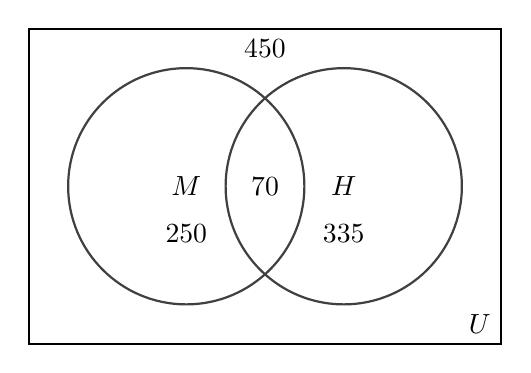
\begin{tikzpicture}[scale=1.0]
	\def\circleA{(0,0) circle (1.5)} %A
	\def\circleB{(0:2) circle (1.5)} %B

	\colorlet{circle edgeA}{black!75} 
	\colorlet{circle areaA}{red!100}
	\colorlet{circle edgeB}{black!75} 
	\colorlet{circle areaB}{green!100}

	\tikzset{
		filledA/.style={fill=circle areaA, draw=circle edgeA, thick},
		filledB/.style={fill=circle areaB, draw=circle edgeB, thick},
		outlineA/.style={draw=circle edgeA, thick},
		outlineB/.style={draw=circle edgeB, thick},
	}

	\begin{scope}[fill opacity=0.5]         
			%\fill[filledB] \circleB;    
			%\fill[filledA] \circleA;
	\end{scope}

	\draw[outlineA] \circleA node {$M$} node[below=10pt] {$250$}; 
	\draw[outlineB] \circleB node {$H$} node[below=10pt] {$335$}; 
	\node at (0:1) {$70$}; %%intersection node%%
	\node[anchor=south] at (current bounding box.north) {$450$}; 
	\draw[thick] (-2,-2) rectangle (4,2) node[anchor=south east] at (current bounding box.south east) {$U$}; 
\end{tikzpicture} 
\end{enumerate}
\item [(b)]$n(H\cap H)=70$
\item [(c)]$n(H-M)=335$
\item [(d)]$n(M\cup H)=250+70+335=655$
\item [(e)]$n\left((M\cup H)'\right)=n(U)-n(M\cup H)=1105-655=450$\vfill
\end{enumerate}
\end{enumerate}
\item \emph{Survivor} and \emph{CSI} belong to the Thursday night prime
time lineup. A group of $600$ college students were surveyed. $350$
students watch \emph{Survivor} and $280$ watch \emph{CSI}. $180$
students watch both shows.

\begin{enumerate}
\item Construct a Venn diagram, and write the appropriate numbers in the
eight regions.
\item How many students watch only \emph{Survivor}?
\item How many students watch \emph{CSI }or \emph{Survivor}?
\item How many students watch only \emph{CSI}?

\begin{enumerate}
\item [(a)]$n(C\cap S)=180$, $n(C-S)=280-180=100$, $n\left(S-C\right)=350-180=170$,
and $n\left((C\cup S)'\right)=600-(180+170+100)=150$

\begin{enumerate}
\item []%%%%A uncolored; B uncolored%%%%%
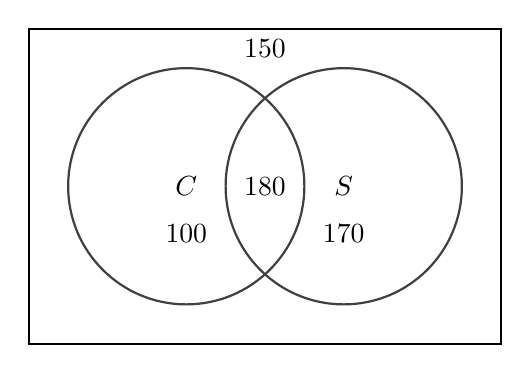
\begin{tikzpicture}[scale=1.0]
	\def\circleA{(0,0) circle (1.5)} %A
	\def\circleB{(0:2) circle (1.5)} %B

	\colorlet{circle edgeA}{black!75} 
	\colorlet{circle areaA}{red!100}
	\colorlet{circle edgeB}{black!75} 
	\colorlet{circle areaB}{green!100}

	\tikzset{
		filledA/.style={fill=circle areaA, draw=circle edgeA, thick},
		filledB/.style={fill=circle areaB, draw=circle edgeB, thick},
		outlineA/.style={draw=circle edgeA, thick},
		outlineB/.style={draw=circle edgeB, thick},
	}

	\begin{scope}[fill opacity=0.5]         
			%\fill[filledB] \circleB;    
			%\fill[filledA] \circleA;
	\end{scope}

	\draw[outlineA] \circleA node {$C$} node[below=10pt] {$100$}; 
	\draw[outlineB] \circleB node {$S$} node[below=10pt] {$170$}; 
	\node at (0:1) {$180$}; %%intersection node%%
	\node[anchor=south] at (current bounding box.north) {$150$}; 
	\draw[thick] (-2,-2) rectangle (4,2) node[anchor=south east] at (current bounding box.south east) {$$}; 
\end{tikzpicture} 
\end{enumerate}
\item [(b)]From diagram: $170$
\item [(c)]From diagram: $n(C\cup S)=100+170+180=450$
\item [(d)]From diagram: $100$
\end{enumerate}
\end{enumerate}
\end{enumerate}
\vfill
\begin{enumerate}[resume]
\item Find the value of each of the following:

\begin{enumerate}
\item $4!$

\begin{enumerate}
\item []$4!=4\cdot3\cdot2\cdot1=24$\newpage
\end{enumerate}
\item $7!$

\begin{enumerate}
\item []$7!=7\cdot6\cdot5\cdot4\cdot3\cdot2\cdot1=5040$
\end{enumerate}
\item $0!$

\begin{enumerate}
\item []$0!=1$
\end{enumerate}
\item $\frac{10!}{7!}$

\begin{enumerate}
\item []$\frac{10!}{7!}=\frac{10\cdot9\cdot8\cdot\cancel{7}\cdot\cancel{6}\cdot\cancel{5}\cdot\cancel{4}\cdot\cancel{3}\cdot\cancel{2}\cdot\cancel{1}}{\cancel{7}\cdot\cancel{6}\cdot\cancel{5}\cdot\cancel{4}\cdot\cancel{3}\cdot\cancel{2}\cdot\cancel{1}}=720$
\end{enumerate}
\item $\frac{27!}{4!25!}$

\begin{enumerate}
\item []$\frac{27!}{4!25!}=\frac{27\cdot26}{4!\cdot1}=\frac{702}{24}=117$.
Similarly to above, everything before $25$ cancels out. 
\end{enumerate}
\item $\frac{1000!}{998!}$

\begin{enumerate}
\item []$\frac{1000!}{998!}=\frac{1000\cdot999}{1}=999,000$. Similarly
to above, everything before $999$ cancels out. 
\end{enumerate}
\item $_{7}P_{2}$

\begin{enumerate}
\item []$_{7}P_{2}=\frac{7!}{(7-2)!}=\frac{7!}{5!}=\frac{5040}{120}=42$
or $\frac{7!}{5!}=7\cdot6=42$.
\end{enumerate}
\item $_{6}C_{4}$

\begin{enumerate}
\item []$_{6}C_{4}=\frac{6!}{(6-4)!4!}=\frac{6!}{2!4!}=\frac{6\cdot5}{2!}=\frac{30}{2}=15$
\end{enumerate}
\end{enumerate}
\end{enumerate}
\vfill
\begin{enumerate}[resume]
\item A certain model of pickup truck is available in five exterior colors,
three interior colors, and three interior styles. In addition, the
transmission can be either manual or automatic, and the truck can
have either two-wheel or four-wheel drive. How many different versions
of the pickup truck can be ordered?

\begin{enumerate}[resume]
\item []We have five categories, $\underline{\,\,\,\,\,}\times\underline{\,\,\,\,\,}\times\underline{\,\,\,\,\,}\times\underline{\,\,\,\,\,}\times\underline{\,\,\,\,\,}$.
Filling in the number of choices for each category we have, 
\[
\underline{5}\times\underline{3}\times\underline{3}\times\underline{2}\times\underline{2}=180
\]
\end{enumerate}
\end{enumerate}
\vfill
\begin{enumerate}[resume]
\item A certain fraternity must elect a president, vice president, and treasurer
from its 30 members. How many ways can this be done?

\begin{enumerate}[resume]
\item []There are no repeats and order does matter (since order will determine
who is pres., vice pres., and treasurer). So we use permutations,
\begin{eqnarray*}
_{30}P_{3}=\frac{30!}{(30-3)!}=\frac{30!}{27!} & = & 30\cdot29\cdot28=24,360
\end{eqnarray*}
\end{enumerate}
\end{enumerate}
\vfill
\begin{enumerate}[resume]
\item A three-person committee must be chosen from a group of ten men and
twelve women. How many committees are possible if it must consist
of the following?

\begin{enumerate}
\item Three men.
\item Three women.
\item One woman and two men.
\item One man and two women.
\item One man and two women, and one of these is selected as a spokesperson
of the committee.

\begin{enumerate}
\item [(a)]No repeats and order doesn't matter$\Rightarrow$combination.
$_{10}C_{3}=\frac{10!}{(10-3)!3!}=\frac{10\cdot9\cdot8}{3!}=\frac{720}{6}=120$
\item [(b)]No repeats and order doesn't matter$\Rightarrow$combination.
$_{12}C_{3}=\frac{12!}{(12-3)!3!}=\frac{12\cdot11\cdot10}{3!}=\frac{1320}{6}=220$
\item [(c)]Here we have two categories: $\underline{\,\,\,\,\,}\times\underline{\,\,\,\,\,}$.
For the first categories we have $12$ choices (equivalently, $_{12}C_{1}=\frac{12!}{(12-1)!1!}=12$),
and for the second we have $_{10}C_{2}=\frac{10!}{(10-2)!2!}=\frac{10\cdot9}{2}=45$.
\\
So we have $12\times45=540$ posibilities.
\item [(d)]Similarly to above, we have two categories. For the first categories
we have $10$ choices, and for the second we have $_{12}C_{2}=\frac{12!}{(12-2)!2!}=\frac{12\cdot11}{2}=66$.
Then we select one of the three to be a spokesperson. \\
So we have $10\times66\times3=1980$ posibilities.
\item []Equivalently, use a permutation where the order of $2$ members
does not matter, $\nicefrac{\left(10\times\frac{12!}{10!}\times3\right)}{2!}=1980$
(like counting the ways to arrange the letters in ``SCHOOL''; the
order of the ``O'''s does not mater).
\end{enumerate}
\end{enumerate}
\end{enumerate}
\vfill
\begin{enumerate}[resume]
\item A card is dealt from a well-shuffled, standard deck of $52$ cards.
Find the probability of being dealt each of the following.\begin{multicols}{2}

\begin{enumerate}
\item A red card

\begin{enumerate}
\item []$\frac{n(\mbox{red cards})}{n(\mbox{cards})}=\frac{26}{52}=\frac{1}{2}$\yspace
\end{enumerate}
\item A queen

\begin{enumerate}
\item []$\frac{n(\mbox{queens})}{n(\mbox{cards})}=\frac{4}{52}=\frac{1}{13}$\yspace
\end{enumerate}
\item A club

\begin{enumerate}
\item []$\frac{n(\mbox{clubs})}{n(\mbox{cards})}=\frac{13}{52}=\frac{1}{4}$\yspace\columnbreak
\end{enumerate}
\item The queen of clubs

\begin{enumerate}
\item []$\frac{n(\mbox{queen of clubs})}{n(\mbox{cards})}=\frac{1}{52}$\yspace
\end{enumerate}
\item A queen or a club

\begin{enumerate}
\item []$\frac{n(\mbox{queens or clubs})}{n(\mbox{cards})}=\frac{4+13-1}{52}=\frac{16}{52}=\frac{4}{13}$\yspace
\end{enumerate}
\item not a queen

\begin{enumerate}
\item []$1-\frac{4}{52}=\frac{48}{52}=\frac{12}{13}$\yspace
\end{enumerate}
\end{enumerate}
\end{multicols}\vfill
\item Three coins are tossed. Find each of the following:\begin{multicols}{2}

\begin{enumerate}
\item the sample space\\
\forestset{  
	L1/.style={rectangle, rounded corners, very     thick},   	
	L2/.style={rectangle, rounded corners, very     thick,
		edge={black,line width=.75pt,line cap=round}},   	
	L3/.style={rectangle, rounded corners, very     thick,
		edge={black,line width=.75pt,line cap=round}},   	
	L4/.style={rectangle, rounded corners, very     thick,
	edge={black,line width=.75pt,line cap=round}}, 
}

\begin{forest}     
	for tree={
		scale=.75,        
		grow=0,
		reversed, %tree direction         
		parent anchor=east,
		child anchor=west, %edge anchors   		edge={line cap=round},
		outer sep=+1pt, %edge/node connection  		rounded corners,
		%minimum width=15mm,
		%minimum height=8mm, %node shape         l 		sep=10mm %level distance     
		}   
[Start,L1
	[H,L2         
		[H,L3            
			[H \{HHH\},L4] 
			[T \{HHT\},L4]         
		]         
		[T,L3          
			[H \{HTH\},L4]
			[T \{HTT\},L4]
		]               
	]
	[T,L2         
		[H,L3            
			[H \{THH\},L4,]
			[T \{THT\},L4,]         
		]         
		[T,L3          
			[H \{TTH\},L4]
			[T \{TTT\},L4]
		]               
	]  
] 
\end{forest}\yspace\columnbreak
\item the event, $E_{1}$, that exactly two are tails

\begin{enumerate}
\item []$E_{1}=\{HTT,THT,TTH\}$\yspace
\end{enumerate}
\item the event, $E_{2}$, that at least two are tails.

\begin{enumerate}
\item []$E_{2}=\{HTT,THT,TTH,TTT\}$\yspace
\end{enumerate}
\item the probability of $E_{1}$

\begin{enumerate}
\item []$p(E_{1})=\frac{3}{8}$\yspace
\end{enumerate}
\item the probability of $E_{2}$

\begin{enumerate}
\item []$p(E_{2})=\frac{4}{8}=\frac{1}{2}$\yspace
\end{enumerate}
\end{enumerate}
\end{multicols}\vfill
\item A drawer has $7$ socks. $4$ socks are black and $3$ are white socks.
John randomly pulls out $4$ socks. Find the probability of the following:\begin{multicols}{2}

\begin{enumerate}
\item all $4$ socks are black.

\begin{enumerate}
\item []$\frac{_{4}C_{4}}{_{7}C_{4}}=\frac{1}{35}$\yspace
\end{enumerate}
\item exactly $2$ are white.

\begin{enumerate}
\item []$\frac{_{3}C_{2}\cdot_{4}C_{2}}{_{7}C_{4}}=\frac{3\cdot6}{35}=\frac{18}{35}$\yspace
\item []$2$ are white and $2$ are black
\end{enumerate}
\columnbreak
\item at least $3$ are white.

\begin{enumerate}
\item []$\frac{_{3}C_{3}\cdot_{4}C_{0}+_{3}C_{4}\cdot_{4}C_{0}}{_{7}C_{4}}=\frac{1\cdot1+0\cdot1}{35}=\frac{1}{35}$\yspace
\item []$3$ OR $4$ are white
\end{enumerate}
\end{enumerate}
\end{multicols}\vfill
\item Of all the flashlights is a large shipment, $15\%$ have a defective
bulb, $10\%$ have a defective battery, and $5\%$ have both defects.
If you buy one of these flashlights, find the probability of the following:\begin{multicols}{2}

\begin{enumerate}
\item a defective bulb or a defective battery

\begin{enumerate}
\item []$p(Batt'\cup Bulb')=.10+.05+.05$
\item []\hspace{0cm}\hphantom{[$p(Batt'\cup Bulb')$}$=.20$\yspace
\end{enumerate}
\item a good bulb or a good battery

\begin{enumerate}
\item []$p((Batt'\cap Bulb'))=1-.05=.95$\yspace
\end{enumerate}
\item a defective bulb and a defective battery. 

\begin{enumerate}
\item []$p(Bulb'\cap Batt')=.05$\yspace
\end{enumerate}
\item just a defective bulb

\begin{enumerate}
\item []$p(Bulb'-Batt')=.10-.05=.05$\yspace\columnbreak
\end{enumerate}
\end{enumerate}
%%%% M or A %%%%%
\begin{center}
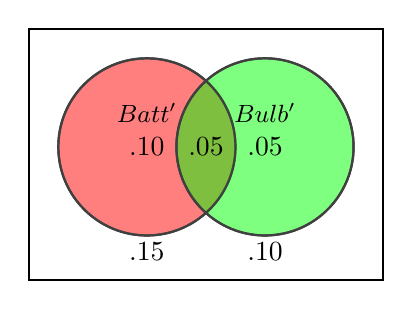
\begin{tikzpicture}[scale=.75]
	\def\circleA{(0,0) circle (1.5)} %A
	\def\circleB{(0:2) circle (1.5)} %B

	\colorlet{circle edgeA}{black!75} 
	\colorlet{circle areaA}{red!100}
	\colorlet{circle edgeB}{black!75} 
	\colorlet{circle areaB}{green!100}

	\tikzset{
		filledA/.style={fill=circle areaA, draw=circle edgeA, thick},
		filledB/.style={fill=circle areaB, draw=circle edgeB, thick},
		outlineA/.style={draw=circle edgeA, thick},
		outlineB/.style={draw=circle edgeB, thick},
	}
	
	\begin{scope}[fill opacity=0.5]         
			\fill[filledA] \circleA;
			\fill[filledB] \circleB;    
	\end{scope}

	\draw[outlineA] \circleA node[above=5pt] {\small $Batt'$} node[] { $.10$} node[below=-1pt] at (0,-1.5) {$.15$}; 
	\draw[outlineB] \circleB node[above=5pt] {\small $Bulb'$} node[] { $.05$} node[below=-1pt] at (2,-1.5) { $.10$};
	\draw (1,0) node {.05};
	\draw[thick] (-2,-2.25) rectangle (4,2) node[anchor=south east] at (current bounding box.south east) {$$}; 
\end{tikzpicture}
\end{center}

\end{multicols}\vfill
\item Use the provided table to answer the following questions.

\begin{tabular}{|c|c|c|c|}
\hline 
\textbf{Age} & \textbf{Obama} & \textbf{McCain} & \textbf{Other/NA}\tabularnewline
\hline 
18-29 & 11.9\% & 5.8\% & 0.4\%\tabularnewline
\hline 
30-44 & 15.1\% & 13.3\% & 0.6\%\tabularnewline
\hline 
45-64 & 18.5\% & 18.1\% & 0.4\%\tabularnewline
\hline 
65+ & 7.2\% & 8.5\% & 0.3\%\tabularnewline
\hline 
\end{tabular}
\begin{enumerate}
\item What is the probability that a voter under $45$ voted for McCain.

\begin{enumerate}
\item []$p(M\mid\mbox{under }45)=\frac{n(M\cap\mbox{under }45)}{n(\mbox{under }45)}=\frac{.058+.133}{.119+.058+.004+.151+.133+.006}=\frac{.191}{.471}\approx40.55\%$\yspace
\end{enumerate}
\item What is the probability that a person who voted for McCain is $45$
or older.

\begin{enumerate}
\item []$p(\mbox{over }45\mid M)=\frac{n(\mbox{over }45\cap M)}{n(M)}=\frac{.181+.085}{.058+.133+.181+.085}=\frac{.266}{.457}\approx58.21\%$\yspace
\end{enumerate}
\end{enumerate}
\vfill
\item Gregor's Garden Corner buys $40\%$ of its plants from the Green Growery
and the rest from Herb's Herbs. Of the plants from the Green Growery,
$20\%$ must be returned, and $10\%$ of those from Herb's Herbs must
be returned. \begin{multicols}{2}

\begin{enumerate}
\item draw a tree diagram describing the probability\\
\tikzset{abovelabel/.style={midway,above,font=\scriptsize}} 
\tikzset{belowlabel/.style={midway,below,font=\scriptsize}} 

\forestset{  
	L1/.style={rectangle, rounded corners, very     thick},   	
	L2/.style={rectangle, rounded corners, very     thick,
		edge={black,line width=.75pt,line cap=round}},   	
	L3/.style={rectangle, rounded corners, very     thick,
		edge={black,line width=.75pt,line cap=round}},   	
	L4/.style={rectangle, rounded corners, very     thick,
	edge={black,line width=.75pt,line cap=round}}, 
}

\begin{forest}     
	for tree={
		scale=1,        
		grow=0,
		reversed, %tree direction         
		parent anchor=east,
		child anchor=west, %edge anchors   		edge={line cap=round},
		outer sep=+1pt, 
		%edge/node connection rounded corners,
		%minimum width=15mm,
		%minimum height=8mm, 
		%node shape
		l sep=1.5cm    
		}   
[Start,L1
	[G,edge label={node[abovelabel]{$.40$}},L2
		[R, edge label={node[abovelabel]{$.20$}}, L3]         
		[R',edge label={node[belowlabel]{$.80$}}, L3]               
	]
	[H,edge label={node[belowlabel]{$.60$}},L2
		[R, edge label={node[abovelabel]{$.10$}}, L3]        
		[R',edge label={node[belowlabel]{$.90$}}, L3]                
	]  
] 
\end{forest}\yspace\vfill\columnbreak
\item find the probability that a plant must be returned and it is from
Herb's Herbs.

\begin{enumerate}
\item []$p(H\cap R)=(.60)(.10)=.06$\yspace
\end{enumerate}
\item find the probability that a plant from the Green Growery must be returned.

\begin{enumerate}
\item []$p(R\mid G)=.20$\yspace
\end{enumerate}
\item find the probability that a plant must be returned. 

\begin{enumerate}
\item []A returned plant can be from Herb's OR Gregory, \\
$p(R)=p(H\cap R)+p(G\cap R)=(.6)(.1)+(.4)(.2)=.06+.08=.14$\yspace
\end{enumerate}
\end{enumerate}
\end{multicols}\vfill
\item Forty randomly selected families were surveyed to determine the number
of children in each family. The following results were found:

\hfill%
\begin{tabular}{cccccccc}
3.7  & 3.6 & 4.0 & 3.8 & 4.1 & 3.9 & 3.5 & 3.9\tabularnewline
3.6 & 4.0 & 3.6 & 3.7 & 3.9 & 3.3 & 3.6 & 4.0\tabularnewline
\end{tabular}\hfill\hspace{0cm}
\begin{enumerate}
\item Find the mean.

\begin{enumerate}
\item []$\bar{x}=\frac{\sum x}{n}=\frac{60.2}{16}\approx3.7625$\vfill
\end{enumerate}
\item Find the median.

\begin{enumerate}
\item []$\frac{3.7+3.8}{2}=3.75$\vfill
\end{enumerate}
\item Find the standard deviation.

\begin{enumerate}
\item []$s=\sqrt{\frac{\sum(x-\bar{x})^{2}}{n-1}}\approx.2217$\vfill
\end{enumerate}
\item Construct a histogram using 5 subintervals, beginning at 3.2, and
ending at 4.2.
\item []\begin{tikzpicture}[scale=.5]
\begin{axis}[     ybar,     ymin=0 ] 
\addplot +[hist={bins=5,data min=3.2,data max=4.2}] table [y index=0] {hist_data_cereal.csv}; 
\end{axis} 
\end{tikzpicture} 
\end{enumerate}
\vfill
\item Find the following probabilities, 

\begin{enumerate}
\item $p(z<1.35)$\begin{multicols}{2}

\begin{enumerate}
\item []$p(z<1.35)\approx91.15\%$ \columnbreak
\item []\normalcdf{0}{1}{-4}{1.35}
\end{enumerate}
\end{multicols}\vfill
\item $p(0<z<2.02)$\begin{multicols}{2}

\begin{enumerate}
\item []$p(0<z<2.02)\approx47.83\%$ \columnbreak
\item []\normalcdf{0}{1}{0}{2.02}
\end{enumerate}
\end{multicols}\vfill
\item $p(-.09<z<1.06)$\begin{multicols}{2}

\begin{enumerate}
\item []$p(-.09<z<1.06)\approx39.13\%$ \columnbreak
\item []\normalcdf{0}{1}{-.09}{1.06}
\end{enumerate}
\end{multicols}\vfill
\item $p(-1.1<z<-.08)$\begin{multicols}{2}

\begin{enumerate}
\item []$p(-1.1<z<-.08)\approx33.25\%$ \columnbreak
\item []\normalcdf{0}{1}{-1.1}{-.08}
\end{enumerate}
\end{multicols}\vfill\newpage
\end{enumerate}
\item A population is normally distributed with a mean 78 and standard deviation
7.5. Find the following probabilities. 

\begin{enumerate}
\item $p(x<70)$\begin{multicols}{2}

\begin{enumerate}
\item []$z_{70}=\frac{70-78}{7.5}=-1.0\bar{6}\approx-1.07$
\item []$p(z<-1.07)\approx14.23\%$ \columnbreak
\item []\normalcdf{78}{7.5}{48}{70}
\end{enumerate}
\end{multicols}\vfill
\item $p(70<x<85)$\begin{multicols}{2}

\begin{enumerate}
\item []$z_{70}\approx-1.07$ and $z_{105}=\frac{85-78}{7.5}\approx.93$
\item []$=p(z<.93)-p(z<-1.07)\approx68.15\%$\columnbreak
\item []$p(-1.07<z<.93)$
\item []\normalcdf{78}{7.5}{70}{85}
\end{enumerate}
\end{multicols}\vfill
\item $p(80<x<95.5)$\begin{multicols}{2}

\begin{enumerate}
\item []$z_{80}=\frac{80-78}{7.5}\approx.27$ and $z_{95.5}=\frac{95.5-78}{7.5}\approx2.33$
\item []$p(.27<z<2.33)$
\item []$=p(z<2.33)-p(z<.27)\approx38.37\%$\columnbreak
\item []\normalcdf{78}{7.5}{80}{95.5}
\end{enumerate}
\end{multicols}\vfill
\item $p(95.5<x<108)$\begin{multicols}{2}

\begin{enumerate}
\item []$z_{95.5}\approx2.33$ and $z_{108}=\frac{108-78}{7.5}=4$
\item []$p(2.33<z<4)$
\item []$=p(z<4)-p(z<2.33)\approx0.99\%$\columnbreak
\item []\normalcdf{78}{7.5}{95.5}{108}
\end{enumerate}
\end{multicols}\vfill
\end{enumerate}
\item Find $c$ such that each of the following is true.

\begin{enumerate}
\item $p(z<c)=0.2776$\begin{multicols}{2}

\begin{enumerate}
\item []$\underset{\mbox{area}}{.2776}\rightarrow\underset{\mbox{z-score}}{-.59}$
\item []$c=-.59$\columnbreak
\item []\normalpdf{0}{1}{-4}{-.59}{-.59}
\end{enumerate}
\end{multicols}\vfill
\item $p(z>c)=.0351$$\leftarrow$area in right tail\begin{multicols}{2}

\begin{enumerate}
\item []Find \emph{z-}score for $1-.0351=.9649$
\item []$\underset{\mbox{area}}{.9649}\rightarrow\underset{\mbox{z-score}}{1.81}$
\item []$c=1.81$\columnbreak
\item []\normalpdf{0}{1}{1.81}{4}{1.81}
\end{enumerate}
\end{multicols}\vfill
\item $p(-c<z<c)=.733$\begin{multicols}{2}

\begin{enumerate}
\item []The area is split on either side of the mean,
\item []Area$=\frac{.733}{2}=.3665$
\item []$\underset{\mbox{area}}{.3665}\rightarrow\underset{\mbox{z-score}}{\pm1.11}$
(using Appendix F)
\item []$c=1.11$ \columnbreak
\item []\normalpdfB{0}{1}{-1.11}{1.11}
\end{enumerate}
\end{multicols}\vfill\newpage
\item Let $\mu=100$ and $\sigma=15$ find $c$ such that $p(x<c)=27.76\%$\begin{multicols}{2}

\begin{enumerate}
\item []$\underset{\mbox{area}}{.2776}\rightarrow\underset{\mbox{z-score}}{-.59}$
\item []$c=\sigma z+\mu\Rightarrow c=15(-.59)+100$
\item []$c=91.15$ \columnbreak
\item []\normalpdf{100}{15}{50}{91.15}{91.15}
\end{enumerate}
\end{multicols}\vfill
\end{enumerate}
\item The time it takes latex paint to dry is normally distributed with
$\mu=3.5$ hours and $\sigma=.75$ hours. Find the probability that
drying time will be as follows.

\begin{enumerate}
\item less than $2.25$ hours.\begin{multicols}{2}

\begin{enumerate}
\item []$z_{2.25}=\frac{2.25-3.5}{.75}=-1.6\bar{6}\approx-1.67$
\item []$p(x<2.25)=p(z<-1.67)=4.75\%$\columnbreak
\item []\normalcdf{3.5}{.75}{.5}{2.25}
\end{enumerate}
\end{multicols}\vfill
\end{enumerate}
\begin{enumerate}[resume]
\item The average score on the ACT is $18$ with a standard deviation of
$6$. If a college only wants to accept students with an ACT score
at least in the top 25\%. What is the minimum score they should accept?
What about the top 5\%?\begin{multicols}{2}

\begin{enumerate}
\item [\textbf{top 25\%:}]$\underset{\mbox{area}}{.75}\rightarrow\underset{\mbox{z-score}}{\approx.67}$
\item []$c=\sigma z+\mu\Rightarrow c=6(.68)+18$
\item []$c=22.08$ 
\item []\normalpdf{18}{6}{22.08}{42}{22.08}\columnbreak
\item [\textbf{top 5\%:}]$\underset{\mbox{area}}{.95}\rightarrow\underset{\mbox{z-score}}{\approx1.645}$
\item []$c=\sigma z+\mu\Rightarrow c=6(1.65)+18$
\item []$c=27.9$ 
\item []\normalpdf{18}{6}{27.9}{42}{27.9}\columnbreak
\end{enumerate}
\end{multicols}\vfill
\end{enumerate}
\end{enumerate}

\end{document}
